% !TEX program = pdflatex

\documentclass[11pt,a4paper]{article}
\usepackage[margin=1in]{geometry}
\usepackage{amsmath, amssymb}
\usepackage{graphicx}

\title{\vspace{-2cm}\textbf{Cross-Domain Clustering for KV-Cache Prefetching}}
\author{Ramblings}  % JOHAIL: rename before this leaves your machine
\date{\today}

\begin{document}
\maketitle

% SECTION ORDER (changed from your draft, reader-dependency reasons):
%   1 Idea & evidence  ->  2 Hub  ->  3 Cost model  ->  4 Bandwidth  ->  5 OOD  ->  6 State map
%   The escape-event definition in the cost model references "hub cluster(s)",
%   so the hub must come first. The bandwidth section consumes f/step, which is
%   produced by the escape simulator in the cost-model section, so it comes after.

\section{General Idea}\label{sec:idea}

KV-cache scaling introduces the problem of cache missing and cache thrashing in LLMs, leading to inefficient processing times for prompts. This memo proposes an offline clustered prefetch architecture that relies on using the attention of a given head at a given layer as a signal for predicting the next cluster needed for evaluating the query.The hypothesis is that there is a learnable graph structure over the clusters formed by the KV vectors in their space. This graph is defined by the flow of attention through these clusters and works like a Markov structure.

The Pythia-410m model was chosen and I focused on layer 13 head 2 of the model. The KV vectors were clustered using K-means over 500-token window lengths and used as the basis for this exploration.

My exploration used this model and tokens from the context of Wikipedia articles and coding prompts. We clustered the KV vectors of this specific head into 64 clusters and noticed that the residuals of the vectors to their centroid displayed a smooth unimodal structure (Figure~\ref{fig:residuals}). An oddity was spotted: a tiny bump near residual $=0.04$ in wiki. Experiments were run to determine whether those tight-fitting keys are the same object as the hub cluster described below (Section~\ref{sec:hub}) or a separate population.

\begin{figure}[h]
\centering
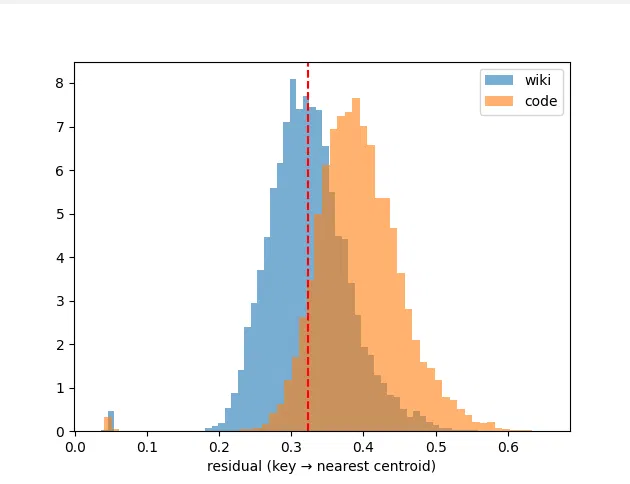
\includegraphics[width=0.72\textwidth]{residual-histogram.png}
% JOHAIL: export the wiki/code residual histogram from your gate1 plotting code
% to figures/residual_hist.png (the one with the 0.04 bump visible).
\caption{Residual distributions (key $\to$ nearest centroid), wiki vs.\ code. Smooth and unimodal on both domains; note the small bump near residual $=0.04$ on wiki, resolved in Section~\ref{sec:hub}.}
\label{fig:residuals}
\end{figure}

Define $d_{val}$ as the mean residual on held-out wiki keys (in-domain) and $d_{code}$ the same on code (out-of-domain), and $D$ as the mean pairwise distance between centroids. These are to check that the wiki-trained centroids do not collapse under OOD data; we want to ensure that the geometry is not meaningless on OOD data, which would materialize as true if the code keys were so far off that they average $d_{code} \approx D$. Data displayed $d_{code}/d_{val} = 1.22$, implying code keys are 22\% further from their nearest centroid than wiki keys: same neighbourhood with tolerable degradation.

We define the transition matrix $A$. $A[i,j]$ counts how often cluster $i$ at step $t-1$ was followed by cluster $j$ at step $t$, within window only. We can normalize our rows to get a Markov kernel of the form $P[i,j] = P(c_t = j \mid c_{t-1} = i)$. Measure the self-loop rate as $\mathrm{trace}(A)/\mathrm{sum}(A) = 0.697$: about 70\% of steps stay in the same cluster. It is also very natural to notice that the graph is directed, with measured off-diagonal asymmetry around 0.607.

$H(c_t)$ measures the entropy: the measure of how surprising it was to see cluster $c$ at step $t$. $H(c_t \mid c_{t-1})$ is the same quantity conditioned on some given information, less than or equal to $H(c_t)$. We use cross-entropy to measure the predictability of cluster trajectories. We computed the empirical cross-entropy on a held-out validation set against an estimated transition model $Q$, built from training-window transition counts with some back-off smoothing for sparse contexts. On order zero (basically the cluster frequencies) we saw a cross-entropy of 5.98 bits, close to the ceiling. When transitioning to an order-1 Markov model by conditioning on the previous cluster, we saw a drop to 2.11 bits. This shows evidence of some temporal structure and proves that the flow of attention could have some predictable sequence.

We measured coverage next: defined as the fraction of the mass that fell inside our resident set of clusters. The setup: you're a prefetcher; you get to keep $k$ clusters resident at any moment; new tokens arrive and their queries attend over past keys. Attention at step $t$ gives a distribution over past keys; group those past keys by cluster and you get a distribution over 64 clusters.

Oracle looks at the true attention mass and keeps the top-$k$ (unbeatable upper bound). Flow graph keeps the top-$k$ clusters predicted by $P_{\text{flow}}[c_{t-1}]$, where $P_{\text{flow}}$ is a matrix trained separately from the transition matrix. It's the average attention destination profile one step after each cluster (indexed by state cluster, not by the attended key cluster). Key graph keeps the top-$k$ from the original $P$ (the key-trajectory kernel). Recency keeps the last $k$ distinct clusters seen --- the null hypothesis that ``attention is just local.'' Static keeps the globally most attended clusters, no dynamics at all --- the null hypothesis that ``one frequency table is enough.'' Position 0 was zeroed out (``sink excluded'') because it always gets massive attention regardless of content, would be pinned resident in any real system, and inflates every method equally, hiding the differences between them.

The table below gives us the results.

{\footnotesize
\begin{verbatim}
--- coverage: wiki held-out, sink excluded (mean attn mass captured, 4990 steps) ---
   k |     oracle | flow_graph |  key_graph |    recency |     static
   1 |      0.759 |      0.217 |      0.217 |      0.217 |      0.217
   2 |      0.917 |      0.800 |      0.265 |      0.348 |      0.788
   4 |      0.985 |      0.951 |      0.396 |      0.433 |      0.815
   8 |      0.997 |      0.986 |      0.454 |      0.494 |      0.839
  16 |      0.999 |      0.995 |      0.462 |      0.589 |      0.891

--- coverage: CODE (OOD, wiki-trained predictors), sink excluded (8483 steps) ---
   k |     oracle | flow_graph |  key_graph |    recency |     static
   1 |      0.682 |      0.198 |      0.198 |      0.198 |      0.198
   2 |      0.873 |      0.668 |      0.253 |      0.331 |      0.686
   4 |      0.965 |      0.867 |      0.386 |      0.438 |      0.716
   8 |      0.990 |      0.936 |      0.478 |      0.519 |      0.751
  16 |      0.998 |      0.967 |      0.499 |      0.606 |      0.830

--- coverage: wiki held-out, sink INCLUDED (reference, 4990 steps) ---
   k |     oracle | flow_graph |  key_graph |    recency |     static
   1 |      0.798 |      0.136 |      0.136 |      0.136 |      0.136
   2 |      0.934 |      0.852 |      0.168 |      0.233 |      0.852
   4 |      0.989 |      0.966 |      0.286 |      0.325 |      0.859
   8 |      0.998 |      0.990 |      0.379 |      0.415 |      0.882
  16 |      1.000 |      0.996 |      0.385 |      0.541 |      0.919
\end{verbatim}
}

We can see the flow graph being close to the oracle (mean gap over $k \in \{2,4,8,16\}$: $0.041$ wiki, $0.097$ code) with the key graph performing poorly. It can also be noted that the flow graph performs better than a static cache. The hub phenomenon (Section~\ref{sec:hub}) goes deeper into a particular bias these results could indicate.


\section{The Hub Phenomenon}\label{sec:hub}

A test was run to identify the most attended-to cluster from the wiki training windows. To make sure that the results from the flow graph were not inflated by constantly predicting this cluster, another test was run where this `hub' cluster (cluster with id 16) was pinned to the resident set and its flow was zeroed out. This showcased whether the flow graph actually contained any predictive structure.

{\footnotesize
\begin{verbatim}
===== pinning 1 hub(s): clusters [16] (train mass share 0.575) =====

--- wiki held-out: hub mass alone 0.573; below = ADDITIONAL from k non-hub residents ---
   k |     oracle | flow_graph |     static
   2 |      0.389 |      0.345 |      0.232
   4 |      0.418 |      0.395 |      0.250
   8 |      0.425 |      0.417 |      0.273

--- code OOD: hub mass alone 0.489; below = ADDITIONAL from k non-hub residents ---
   k |     oracle | flow_graph |     static
   2 |      0.440 |      0.335 |      0.213
   4 |      0.486 |      0.403 |      0.232
   8 |      0.503 |      0.454 |      0.269

===== pinning 2 hub(s): clusters [16, 17] (train mass share 0.607) =====

--- wiki held-out: hub mass alone 0.604; below = ADDITIONAL from k non-hub residents ---
   k |     oracle | flow_graph |     static
   2 |      0.361 |      0.317 |      0.211
   4 |      0.387 |      0.365 |      0.224
   8 |      0.393 |      0.385 |      0.248

--- code OOD: hub mass alone 0.514; below = ADDITIONAL from k non-hub residents ---
   k |     oracle | flow_graph |     static
   2 |      0.419 |      0.318 |      0.202
   4 |      0.463 |      0.385 |      0.217
   8 |      0.478 |      0.433 |      0.257
\end{verbatim}
}

We can see that there is indeed a `hub' in these clusters and that it transfers to OOD as a fixed cluster id. This implies that there is something particularly important about this hub. We also notice that the flow graph has retained its coverage with the loss of the hub as a predictive option and still remains significantly better than the static model and remains close to the oracle (with 1 hub pinned, flow-graph closes 84\% of the static-to-oracle gap on wiki and 67\% on code, averaged over $k \in \{2,4,8\}$; the wiki--code closure gap is the honest OOD degradation of the topology's post-pin edge).

A script was run to identify what keys actually lived in this hub.

Wiki: mostly (space + newline) and other whitespace/punctuation. Small, content-free vocabulary.
Code: 78.8\% of hub keys are the newline token, plus a scattering of other whitespace, punctuation, and a few short identifiers. 33 keys total, which is 0.4\% of all code keys.

Finally, we noticed that every tight-fit key (residual $< 0.1$) lands in cluster 16, implying that the bump in Figure~\ref{fig:residuals} and the hub are the same object. The number of keys that match this description is about 0.44\%, which matches its visual size. Interesting.

% JOHAIL: one interpretation sentence still missing here, and it's the section's
% punchline: the hub is sink-LIKE in function (content-free anchors the model
% parks attention on) but DISTRIBUTED in position, which is why the earlier
% position-histogram defense of the bump as "not sink-like" was wrong for the
% right reason. Standing warnings: do not call it "the attention sink" (that is
% position 0, already excluded), and do not say it "transfers across domains" --
% say the same cluster ID captures similar mass fractions on wiki and code.


\section{The Cost Model and Break-Even}\label{sec:breakeven}

For this entire prediction mechanism to even work, we need to ensure that we beat the base case: a static cache.

Let $h_{static}$ be the hit rate of the required clusters for the decode stage over the resident clusters in the cache, given an attention escape event. An attention escape event occurs iff attention's mass on non-current, non-hub clusters exceeds some threshold. More specifically: on the attention row at step $t$, zero out the mass on the hub cluster(s) and on the state cluster; iff the remaining mass exceeds a threshold, this is an attention escape. Let $h$ be the same hit rate in the proposed prediction paradigm. Let $s$ be the self-loop rate, i.e.\ the probability with which attention remains over the resident clusters. Let $L$ be the latency required to pull non-resident clusters into the cache from DRAM. Let $t$ be the decode time. Let $H$ be the amount of time we spend doing useful work during the predicted fetch in the decode stage in the prediction paradigm. Let us assume that the time taken by the prediction compute is less than the decode time.

A state cluster at time step $t-1$ is the cluster in which the key produced at step $t-1$ fell. The reference pointer is the state cluster whose flow-graph row was consulted to build the current resident set.
% (moved these two definitions up from the end of your draft -- they are used
%  throughout the section, so they belong before first use)

So, this means on a correct fetch for a non-resident cluster in the prediction paradigm, we pay at most $L-H$ time.

The amount of time we spend on every decode stage in the static case is:
\begin{equation*}
    t + (1-s)(1-h_{static})L
\end{equation*}

$h_{static}$ is defined as a conditional that we are moving away from the resident cluster, so the multiplicand cancels out and only leaves the probability that we hit a required non-resident cluster.

The average amount of time we spend in the prediction paradigm is:
\begin{equation*}
    t + (1-s)\left[h\max(0,\, L-H) + (1-h)L\right]
\end{equation*}

So we need
\begin{equation*}
    t + (1-s)\left[h\max(0,\, L-H) + (1-h)L\right] < t + (1-s)(1-h_{static})L
\end{equation*}

Assuming $L-H > 0$, we get
\begin{equation*}
    hH/L > h_{static}
\end{equation*}

If we assume that $L-H < 0$, we get $h > h_{static}$. Therefore, combining the cases we get
\begin{equation*}
    h \min(1,\, H/L) > h_{static}
\end{equation*}

Looking more closely at the model: assuming a 7B-class MHA, with head dim 128, 128k context, per head per layer, DRAM tier. Assuming $t \approx 33$ ms (which is 30 tok/s) gives us $L/t \approx 0.008$, assuming $L \approx 0.26$ ms. Setting $H = mt$, with $m = 8$, we get $\min(1, H/L) = \min(1, \approx\!10^3) = 1$. So our inequality just collapses to $h > h_{static}$. Latency is not the constraint, prediction quality is.
% (adjusted L from 0.21 to 0.26 ms so L/t = 0.008 is internally consistent;
%  0.21/33 gives 0.0064. Either pair is defensible -- pick one and it must agree.)

The table below measures both sides of the inequality directly, conditional on the escape event, with the hub (cluster 16) pinned. THRESH is the escape threshold; $m$ is the refresh interval of the staged set; ev is the event-driven refresh mode described below.

{\footnotesize
\begin{verbatim}
--- wiki held-out ---   [THRESH = 0.25, HUBS = (16,)]
    k    m |   esc% |   h_esc h_st_esc |   h_all h_st_all |  f/ref  f/step
    2    1 |  28.0% |   0.708    0.089 |   0.597    0.036 |   0.34   0.340
    2    8 |  28.0% |   0.776    0.089 |   0.667    0.036 |   0.88   0.112
    2   16 |  28.0% |   0.692    0.089 |   0.628    0.036 |   1.36   0.087
    2   ev |  28.0% |   0.708    0.089 |   0.597    0.036 |   1.13   0.340
    4    1 |  28.0% |   0.923    0.176 |   0.862    0.083 |   0.42   0.419
    4    8 |  28.0% |   0.925    0.176 |   0.862    0.083 |   1.10   0.139
    4   16 |  28.0% |   0.874    0.176 |   0.810    0.083 |   1.94   0.124
    4   ev |  28.0% |   0.923    0.176 |   0.862    0.083 |   1.39   0.419
    8    1 |  28.0% |   0.976    0.290 |   0.963    0.183 |   0.62   0.623
    8    8 |  28.0% |   0.978    0.290 |   0.955    0.183 |   1.77   0.223
    8   16 |  28.0% |   0.956    0.290 |   0.928    0.183 |   2.86   0.183
    8   ev |  28.0% |   0.976    0.290 |   0.963    0.183 |   2.07   0.623

--- code OOD ---   [THRESH = 0.25, HUBS = (16,)]
    k    m |   esc% |   h_esc h_st_esc |   h_all h_st_all |  f/ref  f/step
    2    1 |  42.7% |   0.518    0.053 |   0.499    0.046 |   0.44   0.437
    2    8 |  42.7% |   0.561    0.053 |   0.553    0.046 |   0.98   0.123
    2   16 |  42.7% |   0.516    0.053 |   0.525    0.046 |   1.37   0.088
    2   ev |  42.7% |   0.518    0.053 |   0.499    0.046 |   1.20   0.437
    4    1 |  42.7% |   0.717    0.117 |   0.732    0.108 |   0.57   0.569
    4    8 |  42.7% |   0.726    0.117 |   0.738    0.108 |   1.36   0.172
    4   16 |  42.7% |   0.684    0.117 |   0.694    0.108 |   2.06   0.132
    4   ev |  42.7% |   0.717    0.117 |   0.732    0.108 |   1.56   0.569
    8    1 |  42.7% |   0.860    0.229 |   0.901    0.219 |   0.90   0.898
    8    8 |  42.7% |   0.861    0.229 |   0.888    0.219 |   2.12   0.268
    8   16 |  42.7% |   0.844    0.229 |   0.857    0.219 |   3.13   0.201
    8   ev |  42.7% |   0.860    0.229 |   0.901    0.219 |   2.46   0.898
\end{verbatim}
}

At $k=4$ in ev mode: wiki $h_{esc} = 0.923$ vs $h_{st,esc} = 0.176$ (a $5.2\times$ margin); code $0.717$ vs $0.117$ (a $6.1\times$ margin). The pattern is threshold-insensitive across thresholds in $\{0.10, 0.25, 0.50\}$.

Looking now at the original coverage table, we see a couple of flaws. Firstly, the static case had inflations in scores, since the self-loop steps where nothing needed to be fetched, and the steps when the hubs were hit while resident, resulted in false coverage. Under the new conditional, we can see the break-even margin is far higher.

Furthermore, we previously saw an ON-DEMAND policy winning out when $k=2$ and $m=16$ (wiki: $h_{staged} = 0.531 < h_{static} = 0.654$; code: $0.487 < 0.537$). However, under the conditioning, this anomaly vanishes. This occurred before because the static policy's guaranteed-fresh cluster was working against an extremely stale flow-graph snapshot (the state would have been expected to move with probability $1 - 0.697^{16} \approx 0.997$ by then). The conditioning zeroes this out and the fresh slot is not counted in the score anymore.

Finally, another interesting artifact is that $m=8 > m=1$. At THRESH $=0.25$ on wiki data at $k=2$: $h_{esc}(m{=}1) = 0.708$, $h_{esc}(m{=}8) = 0.776$; $m=8$ beats $m=1$ by $0.068$. Similar at $k=4$: $0.923$ vs $0.925$ (small but positive). This is likely because the seed slot of $m=1$ always holds the previous time step's state cluster, which is zeroed under the conditioning, making it worthless for the scoring. At $m=8$ the seeded slot holds the old reference pointer from up to 8 steps ago. When attention does escape back to that cluster, the $m=8$ frozen set catches it; the $m=1$ policy does not, since we only zero out the last step's cluster.
% (numbers in this paragraph corrected to the canonical HUBS=(16,) run; your
%  draft quoted 0.695/0.770 and 0.919/0.923, which are from the (16,17) run)

An event-driven (ev) refresh mode was also tested. In this mode, the resident set is recomputed only when the state cluster changes from the reference pointer. This produces the same results (resident sets, hit rates, and bandwidth) as the $m=1$ regime at every step. This is because the reference pointer is the same as the live state pointer under both policies; the only difference being that the compute for self-loops is avoided in the ev case. Another interesting note is that even under a pointer change, the resident set may not change, if the new row's predicted cluster set and the current resident set's intersection is the predicted cluster set. This is the smoothness property of the row map.


\section{System Scope and Hardware Constraints}\label{sec:bandwidth}

The PCIe bus has a fixed budget in bytes/second. Our design cannot fetch so much data that it saturates the bus (this makes our inequality moot, since the latency is assumed a constant, not a load-bearing quantity). We measured $f/\text{step}$, the mean number of clusters fetched per decode step. Assuming a 30 tokens/second decode rate, we get $30 \cdot f/\text{step}$ clusters/second per graph.

KV per token per head-layer $= (2)(128)(2) = 512$~B. One head-layer's cache at 128k context is $\approx 67$~MB; one cluster $\approx 1.05$~MB; a $k=4$ staged fetch $\leq 4.2$~MB.

This means we have $30 \cdot (f/\text{step}) \cdot 1.05$ MB/second per graph. Assuming our PCIe budget is 20~GB/second, we can fit a different number of graphs into our model depending on our cluster count and refresh rate. The table below gives the number of head-layer graphs that fit in the budget, using the measured $f/\text{step}$ values from the escape simulator (HUBS $=(16,)$).

{\footnotesize
\begin{verbatim}
graphs that fit in a 20 GB/s PCIe budget  (G = 20000 / (31.5 * f/step))

                    wiki                          code
   k |   m=1 (=ev)     m=8    m=16 |   m=1 (=ev)     m=8    m=16
   2 |        1867    5669    7298 |        1453    5162    7215
   4 |        1515    4568    5120 |        1116    3691    4810
   8 |        1019    2847    3470 |         707    2369    3159

old full-refresh accounting (4.2 MB x 8 refreshes/s = 33.6 MB/s):  ~595 graphs
a 32L x 32H model has 1024 head-layer combinations
\end{verbatim}
}

% JOHAIL: your ev discussion goes here, plus the conclusion rewrite this table
% forces: at k=4 the ENTIRE 1024 head-layer model now fits under budget at every
% refresh policy, on both domains -- delta-fetch accounting flips the old
% "deeper layers only" necessity into a k=8 / headroom choice. The pipeline
% lead-time argument for deeper layers survives as a bonus, not a constraint.


\section{Cross-Domain Transfer (OOD)}\label{sec:ood}
% JOHAIL: yours to write -- the section is two SEPARATE claims; do not conflate:
%
% Claim 1 (token-level pinning transfer): pinning cluster 16 transfers because
%   the hub anchors tokenizer-level function tokens (newline, whitespace,
%   punctuation) that appear in every domain. Evidence: hub mass 0.573 wiki /
%   0.489 code as a FIXED cluster id; token tables in Section 2. Cheap claim,
%   strong evidence -- the tokenizer almost guarantees it.
%
% Claim 2 (topological transfer): the flow graph's post-pin edge transfers by a
%   DIFFERENT mechanism, which is uncharacterized. Evidence: +0.395 wiki vs
%   +0.403 code additional mass at k=4 with wiki-trained predictors -- near
%   equal. This cannot be Claim 1's mechanism because the hubs are excluded
%   from both the predictions and the scored mass. Candidate mechanisms
%   (shared syntax, low-level token patterns, geometric structure) are
%   untested -- state that openly.


\section{Ambiguity, Staleness, and the State Map}\label{sec:statemap}

When a key gets mapped to a centroid, the closest one in distance ($d_1$) is chosen. An `ambiguous' choice is one where $d_1/d_2 > 0.9$: the two centroids are nearly tied in distance, making the argmax a coin flip. We can split the classifications into ambiguous and controls.

We can now build candidate staged sets using this. $S_1$ is the top-$k$ of $P_{\text{flow}}[c_1]$, where $c_1$ was the argmax cluster; the prefetcher would stage this. $S_2$ is the same for $c_2$. We also define $S_s$, a soft mixture of the two with priority given to $c_1$.

We can measure the Jaccard similarity on these sets, and the actual attention mass at step $t$ that falls into each of the three sets. This is the term that the break-even cares about. The Jaccard similarity measures how much overlap exists between adjacent clusters' rows in $P_{\text{flow}}$, and the mass captured measures the cost we would pay if we use the wrong row.

We predicted a relatively high identical rate on ambiguous, about 70\%, and lower on the control. This was justified by the notion of row smoothness, where nearby centroids should have similar flow rows. However, we saw something outstanding: 5.9\% identical on wiki ambiguous, 6.0\% on control.

{\footnotesize
\begin{verbatim}
--- wiki held-out ---
 ambiguous (n=1625): identical 5.9% jaccard 0.504 
   | mass: argmax 0.389 runner-up 0.361 soft 0.400
   
 control (n=3365): identical 6.0% jaccard 0.494 
   | mass: argmax 0.398 runner-up 0.329 soft 0.397

--- code OOD ---
 ambiguous (n=4991): identical 5.1% jaccard 0.450 
   | mass: argmax 0.384 runner-up 0.335 soft 0.394
   
 control (n=3492): identical 4.9% jaccard 0.475 
   | mass: argmax 0.430 runner-up 0.350 soft 0.429
\end{verbatim}
}

For the two sets to be identical we would require a really strong condition: $c_2$ would have to be in the top-$k$ of $c_1$'s row and vice versa --- mutual top rank from both seeds. Since $c_1 \neq c_2$, the Jaccard of two staged sets built from \emph{identical} rows is bounded by $(k-1)/(k+1)$, which is $0.6$ at $k=4$. The observed similarity of $0.504$ is 84\% of that ceiling. We were looking at the wrong observable.
% (corrected: your draft had 0.667 and "76% of the way" -- the ceiling is
%  (k-1)/(k+1) = 3/5 = 0.6 because the union has k+1 elements, not k+2;
%  only the two seeds differ. 0.504/0.6 = 0.84.)

We also see that the wrong-row penalty scales with the key distance (argmax minus runner-up mass: wiki $0.028$ ambiguous vs $0.069$ control; code $0.049$ vs $0.080$). Soft assignment recovers a small amount of mass in the ambiguous case, essentially none on control. We can deduce that we have a locally smooth structure that is non-degenerate globally. In other words, small pointer perturbations produce small changes and larger ones produce appropriately larger changes.

Another interesting point has to do with the exact type of perturbation. Ambiguity perturbs through noise, whereas staleness perturbs through time. We can compute coverage as a function of pointer distance and Jaccard as a function of centroid distance. If the curves collapse, we have some sort of isomorphism between the two. I predict that the curves will agree for smaller perturbations, but for larger ones the similarity will decay faster than coverage. Temporal locality is really strong in this case, as observed by the excursion-return idea in the previous paragraphs.

{\footnotesize
\begin{verbatim}
staleness sweep (Test F): flow_graph coverage at k=4, staged set refreshed every m steps
  wiki held-out:  m=1  0.951    m=8  0.915    m=16  0.862    m=32  0.765
  code OOD:       m=1  0.867    m=8  0.828    m=16  0.776    m=32  0.695
\end{verbatim}
}
% JOHAIL: paste the full sweep (m=2, 4 rows included) if you want the whole curve.
% JOHAIL TODO -- still unwritten, and it is this section's original purpose:
% reconcile the 94% stale-pointer rate at m=8 (s^8 = 0.056) with the flat curve
% above. Two mechanisms, both yours from earlier: the hub-caught FLOOR (hub is
% in every staged set) and the row-map smoothness RATE mechanism (a stale
% pointer still points at approximately the right set). Write the paragraph.

\end{document}